\documentclass[tikz,border=2pt]{standalone}
\usepackage{amsmath,amssymb}
\usepackage{pgfplots}
\pgfplotsset{compat=1.18}

\begin{document}
% F(x, y) = P(X <= x, Y <= y) collects the probability to the lower left of (x, y). Independent
% uniforms: the area 0.4 * 0.5. Y = X: all mass on the diagonal, the part up to 0.4.
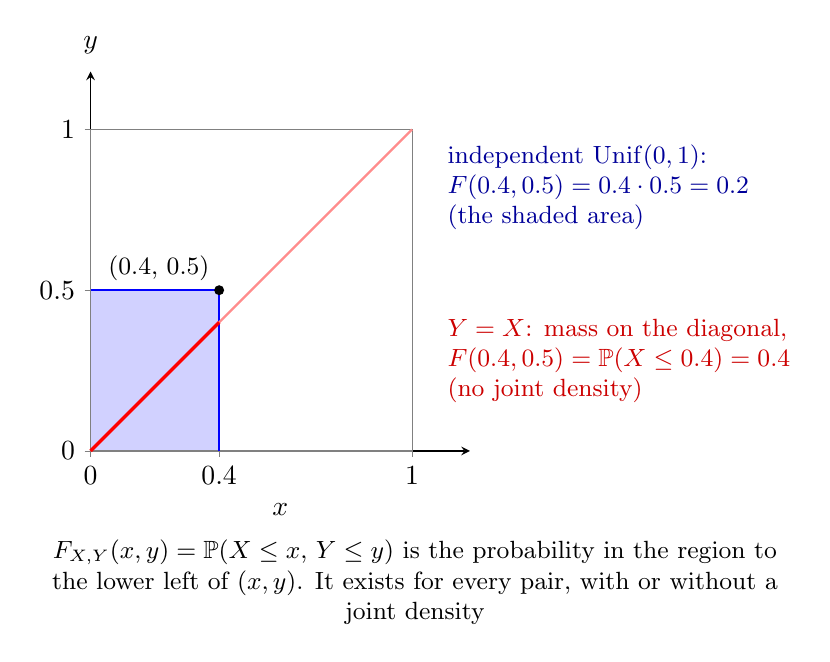
\begin{tikzpicture}
	\begin{axis}[
		axis lines=left, xmin=0, xmax=1.18, ymin=0, ymax=1.18,
		xtick={0,0.4,1}, ytick={0,0.5,1},
		xlabel={$x$}, ylabel={$y$}, ylabel style={rotate=-90, anchor=south, at={(axis description cs:0,1.02)}},
		width=6.4cm, height=6.4cm, clip=false
		]
		\fill[blue!18] (axis cs:0,0) rectangle (axis cs:0.4,0.5);
		\draw[gray] (axis cs:0,0) rectangle (axis cs:1,1);
		\draw[blue, thick] (axis cs:0.4,0) -- (axis cs:0.4,0.5) -- (axis cs:0,0.5);
		\draw[red!45, thick] (axis cs:0,0) -- (axis cs:1,1);
		\draw[red, very thick] (axis cs:0,0) -- (axis cs:0.4,0.4);
		\fill[black] (axis cs:0.4,0.5) circle (1.8pt);
		\node[anchor=south east, font=\small] at (axis cs:0.4,0.5) {$(0.4,\,0.5)$};
		\node[blue!60!black, anchor=west, font=\small, align=left] at (axis cs:1.08,0.82) {independent $\operatorname{Unif}(0,1)$:\\ $F(0.4,0.5)=0.4\cdot0.5=0.2$\\ (the shaded area)};
		\node[red!80!black, anchor=west, font=\small, align=left] at (axis cs:1.08,0.28) {$Y=X$: mass on the diagonal,\\ $F(0.4,0.5)=\mathbb{P}(X\le0.4)=0.4$\\ (no joint density)};
	\end{axis}
	\node[anchor=north, font=\small, align=flush center, text width=9.6cm] at ([yshift=-2pt]current axis.outer south) {$F_{X,Y}(x,y)=\mathbb{P}(X\le x,\,Y\le y)$ is the probability in the region to the lower left of $(x,y)$. It exists for every pair, with or without a joint density};
\end{tikzpicture}
\end{document}
